\documentclass[dvipdfmx,titlepage,a4j]{jsarticle}

\usepackage[top=20mm,bottom=20mm,left=20mm,right=20mm]{geometry}


\usepackage{url}
\usepackage{graphicx}
\usepackage{listings,jvlisting}
\usepackage{amsmath,amssymb}
\usepackage{graphicx}
\usepackage[yen]{okuverb}
\usepackage{ascmac}
\usepackage{fancybox}
\usepackage{fancyvrb}
\usepackage{fancyhdr}
\usepackage{lastpage}
\usepackage{caption}
\usepackage{subcaption}
\usepackage{here}
\usepackage{titling}

% ヘッダーとフッターの設定
\renewcommand{\headrulewidth}{0.2pt} % ヘッダーの線
\renewcommand{\footrulewidth}{0.4pt} % フッターの線

% ヘッダー 
\fancyhead[L]{}
\fancyhead[C]{\thetitle}
\fancyhead[R]{}

% フッター
\fancyfoot[L]{}
\fancyfoot[C]{\thepage / \pageref{LastPage}} % ページ番号
\fancyfoot[R]{}

% lstlistingの設定
\lstset{
  language={C++},
  basicstyle={\ttfamily},
  identifierstyle={\small},
  commentstyle={\smallitshape},
  keywordstyle={\small\bfseries},
  ndkeywordstyle={\small},
  stringstyle={\small\ttfamily},
  frame={tb},
  tabsize={2},
  breaklines=true,
  columns=[l]{fullflexible},
  numbers=left,
  xrightmargin=0zw,
  xleftmargin=3zw,
  numberstyle={\scriptsize},
  stepnumber=1,
  numbersep=1zw,
  lineskip=-0.5ex
}

\title{超小型衛星向け光学ミッション設計の教科書}
\author{waarrk}
\date{2023年2月1日}

\begin{document}

\begin{titlepage}
    \centering
    \vspace*{2cm}

    \vspace{5cm}

    {\LARGE \textbf{小惑星表面探査を想定したCubeSat放出機構を使用して\\運用可能な多脚式自律移動ロボットの開発}}

    \vspace{0.5cm}

    {\textbf{千葉工業大学 先進工学部 未来ロボティクス学科}\\}
    {\textbf{22C1704 鷲尾 優作}}

    \vfill

    {\large 2025年5月7日}

    \vspace{1cm}
\end{titlepage}

\newpage

\section{目的}
本計画書は、修士課程の研究計画を明確化し、指導教員との合意形成を図ることを目的とする。

\section{研究背景}
近年、小惑星探査は、地球衝突天体への対処(いわゆるプラネタリーディフェンス)や、
宇宙資源の活用を目的とした探査の観点から、注目を集めている。

小惑星探査機は、サンプル採取ミッションを除き、探査機本体へのリスクを最小化するため、小惑星表面に極端に接近することは避け、観測は主に上空からのリモートセンシングで行う。
したがって、表面の微細構造の解析には限界がありこの観測のため、日本の「はやぶさ2」では、小惑星表面にロボットを投下する試みが行われている。
MINERVA-II1A/B\cite{minelva:online}およびMASCOT\cite{Krause2022}は、表面画像やデータ取得に成功し、成果を挙げた(図\ref{fig:hayabusa2})。

\begin{figure}[H]
    \centering
    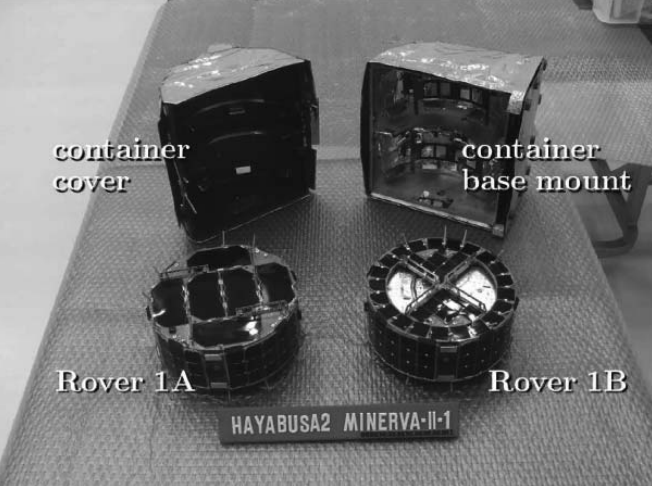
\includegraphics[width=0.5\textwidth]{picture/mine.png}
    \caption{「はやぶさ2」に搭載されたロボット「MINERVA-II-1」}
    \label{fig:hayabusa2}
\end{figure}

MINERVAシリーズはホッピング機構によって移動可能であったものの、
任意の目標に移動する機能は備えておらず、その移動は跳躍によるもので軌道制御には限界があった。
これらのロボットは、いずれも実証的かつ専用設計であり、他ミッションへの汎用的な転用はなされていない。

小惑星表面探査機は、表面の任意の地点でデータを取得できることが理想であるが、
微小重力環境かつ不整地であるため、そもそも移動以前に目的位置への着地自体が高難度である。
初代はやぶさに搭載されたMINERVA\cite{探査ロボット「ミ5:online}は、放出時の方向不良により行方不明となったほか、
欧州の彗星探査機ロゼッタに搭載された着陸機フィラエ\cite{ESARoset23:online}でも、目的位置で固定するアンカーの作動不良により大きく外れた位置に着地するなどのトラブルが発生している。
機構の簡素化を重視した結果、固定・移動機能の実装が見送られてきた傾向もある。

この課題に対する解決策として、2つの方向性が挙げられる。
探査機の台数を増やし観測点を分散させることで、着地地点の不確実性を軽減する方法、
各探査機に自律的な移動機能を付与し、着地後でも自ら有利な観測地点へ移動できるようにする方法である。

一方、近年、CubeSatに代表される超小型衛星の普及により、宇宙開発における低コスト化と短期開発が進んでいる。
CubeSatは、1U(10cm立方)を基本単位とした規格に基づいて設計されており、主に低軌道における実績を積み重ねてきた。
近年では、こうした小型衛星が深宇宙探査にも応用されつつあり、欧州宇宙機関(ESA)の小惑星探査機「Hera」では2機のCubeSatが搭載された\cite{ESAHeraa1:online}。

また、小惑星探査機そのものも民間参入の流れがあり、マクサー社製の小惑星探査機「サイキ」がすでに打ち上げられているほか、
2028年にはExLabs社の「SERV」が、千葉工業大学製のCubeSat放出型の小型探査機(非移動型)を搭載し打ち上げられる予定である。

これらの背景から、CubeSatのサイズ準拠した脚などの移動機構を備えたロボットを開発すれば、先の小惑星表面探査機の課題を解決できる可能性がある。
共通設計によるコスト削減や、放出機構の流用による開発期間の短縮が期待できる。

\section{研究目的}
CubeSat放出機構から放出可能な多脚式自律移動ロボットを開発し、
小惑星表面における多点観測を実現可能とする移動探査技術の確立を目指す。

\section{研究内容}
本研究では、以下の2点を中心に取り組む。

\begin{enumerate}
    \item \textbf{機体設計:}
          CubeSat放出機構に収容可能な多脚型機構を設計する。
    \item \textbf{自律制御系:}
          ロボットの搭載コンピュータ上に何らかのナビゲーションを実装し、任意の観測地点への経路計画を目指す。
\end{enumerate}

設計・開発は、2025年度に実施する小惑星アポフィス向け探査機の設計知見を踏まえ、後継機としての要求仕様を随時反映しつつ進める。


\section{研究スケジュール}
2025年4月から学部4年時に先行機の設計を行い、2026年4月から修士課程に進学後、移動型ロボット試作機の構想設計を行う。
修士課程入学後は、宇宙科学技術連合講演会、IROS、アストロダイナミクスシンポジウム等の学会において、研究成果を発表する。

\begin{table}[H]
    \centering
    \caption{スケジュール案}
    \begin{tabular}{l|l}
        \hline
        期間           & 内容           \\
        \hline \hline
        2025年4月から12月 & 先行機の開発       \\
        \hline
        2026年1月から3月  & 具体的な後継機の仕様検討 \\
        \hline
        2026年4月頃から   & 試作機構造設計      \\
        \hline
        2027年4月頃から   & 試作機ソフトウェア設計  \\
        \hline
        2027年頃       & 学会発表         \\
        \hline
    \end{tabular}
    \label{tab:schedule}
\end{table}

\section{期待される成果}
CubeSat放出機構と組み合わせて運用可能な自律移動ロボットの試作機が完成する見込みである。将来的には、小惑星表面での観測を支える技術としての活用が期待できる。

\newpage

\nocite{*}
\bibliographystyle{jplain}
\bibliography{refs}

\end{document}
